\documentclass[1p]{elsarticle_modified}
%\bibliographystyle{elsarticle-num}

%\usepackage[colorlinks]{hyperref}
%\usepackage{abbrmath_seonhwa} %\Abb, \Ascr, \Acal ,\Abf, \Afrak
\usepackage{amsfonts}
\usepackage{amssymb}
\usepackage{amsmath}
\usepackage{amsthm}
\usepackage{scalefnt}
\usepackage{amsbsy}
\usepackage{kotex}
\usepackage{caption}
\usepackage{subfig}
\usepackage{color}
\usepackage{graphicx}
\usepackage{xcolor} %% white, black, red, green, blue, cyan, magenta, yellow
\usepackage{float}
\usepackage{setspace}
\usepackage{hyperref}

\usepackage{tikz}
\usetikzlibrary{arrows}

\usepackage{multirow}
\usepackage{array} % fixed length table
\usepackage{hhline}

%%%%%%%%%%%%%%%%%%%%%
\makeatletter
\renewcommand*\env@matrix[1][\arraystretch]{%
	\edef\arraystretch{#1}%
	\hskip -\arraycolsep
	\let\@ifnextchar\new@ifnextchar
	\array{*\c@MaxMatrixCols c}}
\makeatother %https://tex.stackexchange.com/questions/14071/how-can-i-increase-the-line-spacing-in-a-matrix
%%%%%%%%%%%%%%%

\usepackage[normalem]{ulem}

\newcommand{\msout}[1]{\ifmmode\text{\sout{\ensuremath{#1}}}\else\sout{#1}\fi}
%SOURCE: \msout is \stkout macro in https://tex.stackexchange.com/questions/20609/strikeout-in-math-mode

\newcommand{\cancel}[1]{
	\ifmmode
	{\color{red}\msout{#1}}
	\else
	{\color{red}\sout{#1}}
	\fi
}

\newcommand{\add}[1]{
	{\color{blue}\uwave{#1}}
}

\newcommand{\replace}[2]{
	\ifmmode
	{\color{red}\msout{#1}}{\color{blue}\uwave{#2}}
	\else
	{\color{red}\sout{#1}}{\color{blue}\uwave{#2}}
	\fi
}

\newcommand{\Sol}{\mathcal{S}} %segment
\newcommand{\D}{D} %diagram
\newcommand{\A}{\mathcal{A}} %arc


%%%%%%%%%%%%%%%%%%%%%%%%%%%%%5 test

\def\sl{\operatorname{\textup{SL}}(2,\Cbb)}
\def\psl{\operatorname{\textup{PSL}}(2,\Cbb)}
\def\quan{\mkern 1mu \triangleright \mkern 1mu}

\theoremstyle{definition}
\newtheorem{thm}{Theorem}[section]
\newtheorem{prop}[thm]{Proposition}
\newtheorem{lem}[thm]{Lemma}
\newtheorem{ques}[thm]{Question}
\newtheorem{cor}[thm]{Corollary}
\newtheorem{defn}[thm]{Definition}
\newtheorem{exam}[thm]{Example}
\newtheorem{rmk}[thm]{Remark}
\newtheorem{alg}[thm]{Algorithm}

\newcommand{\I}{\sqrt{-1}}
\begin{document}

%\begin{frontmatter}
%
%\title{Boundary parabolic representations of knots up to 8 crossings}
%
%%% Group authors per affiliation:
%\author{Yunhi Cho} 
%\address{Department of Mathematics, University of Seoul, Seoul, Korea}
%\ead{yhcho@uos.ac.kr}
%
%
%\author{Seonhwa Kim} %\fnref{s_kim}}
%\address{Center for Geometry and Physics, Institute for Basic Science, Pohang, 37673, Korea}
%\ead{ryeona17@ibs.re.kr}
%
%\author{Hyuk Kim}
%\address{Department of Mathematical Sciences, Seoul National University, Seoul 08826, Korea}
%\ead{hyukkim@snu.ac.kr}
%
%\author{Seokbeom Yoon}
%\address{Department of Mathematical Sciences, Seoul National University, Seoul, 08826,  Korea}
%\ead{sbyoon15@snu.ac.kr}
%
%\begin{abstract}
%We find all boundary parabolic representation of knots up to 8 crossings.
%
%\end{abstract}
%\begin{keyword}
%    \MSC[2010] 57M25 
%\end{keyword}
%
%\end{frontmatter}

%\linenumbers
%\tableofcontents
%
\newcommand\colored[1]{\textcolor{white}{\rule[-0.35ex]{0.8em}{1.4ex}}\kern-0.8em\color{red} #1}%
%\newcommand\colored[1]{\textcolor{white}{ #1}\kern-2.17ex	\textcolor{white}{ #1}\kern-1.81ex	\textcolor{white}{ #1}\kern-2.15ex\color{red}#1	}

{\Large $\underline{12a_{0586}~(K12a_{0586})}$}

\setlength{\tabcolsep}{10pt}
\renewcommand{\arraystretch}{1.6}
\vspace{1cm}\begin{tabular}{m{100pt}>{\centering\arraybackslash}m{274pt}}
\multirow{5}{120pt}{
	\centering
	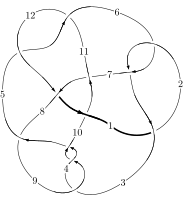
\includegraphics[width=112pt]{../../../GIT/diagram.site/Diagrams/png/1387_12a_0586.png}\\
\ \ \ A knot diagram\footnotemark}&
\allowdisplaybreaks
\textbf{Linearized knot diagam} \\
\cline{2-2}
 &
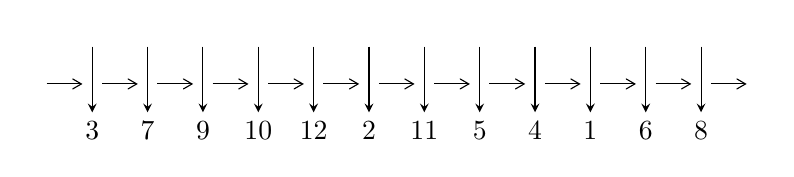
\begin{tikzpicture}[x=20pt, y=17pt]
	% nodes
	\node (C0) at (0, 0) {};
	\node (C1) at (1, 0) {};
	\node (C1U) at (1, +1) {};
	\node (C1D) at (1, -1) {3};

	\node (C2) at (2, 0) {};
	\node (C2U) at (2, +1) {};
	\node (C2D) at (2, -1) {7};

	\node (C3) at (3, 0) {};
	\node (C3U) at (3, +1) {};
	\node (C3D) at (3, -1) {9};

	\node (C4) at (4, 0) {};
	\node (C4U) at (4, +1) {};
	\node (C4D) at (4, -1) {10};

	\node (C5) at (5, 0) {};
	\node (C5U) at (5, +1) {};
	\node (C5D) at (5, -1) {12};

	\node (C6) at (6, 0) {};
	\node (C6U) at (6, +1) {};
	\node (C6D) at (6, -1) {2};

	\node (C7) at (7, 0) {};
	\node (C7U) at (7, +1) {};
	\node (C7D) at (7, -1) {11};

	\node (C8) at (8, 0) {};
	\node (C8U) at (8, +1) {};
	\node (C8D) at (8, -1) {5};

	\node (C9) at (9, 0) {};
	\node (C9U) at (9, +1) {};
	\node (C9D) at (9, -1) {4};

	\node (C10) at (10, 0) {};
	\node (C10U) at (10, +1) {};
	\node (C10D) at (10, -1) {1};

	\node (C11) at (11, 0) {};
	\node (C11U) at (11, +1) {};
	\node (C11D) at (11, -1) {6};

	\node (C12) at (12, 0) {};
	\node (C12U) at (12, +1) {};
	\node (C12D) at (12, -1) {8};
	\node (C13) at (13, 0) {};

	% arrows
	\draw[->,>={angle 60}]
	(C0) edge (C1) (C1) edge (C2) (C2) edge (C3) (C3) edge (C4) (C4) edge (C5) (C5) edge (C6) (C6) edge (C7) (C7) edge (C8) (C8) edge (C9) (C9) edge (C10) (C10) edge (C11) (C11) edge (C12) (C12) edge (C13) ;	\draw[->,>=stealth]
	(C1U) edge (C1D) (C2U) edge (C2D) (C3U) edge (C3D) (C4U) edge (C4D) (C5U) edge (C5D) (C6U) edge (C6D) (C7U) edge (C7D) (C8U) edge (C8D) (C9U) edge (C9D) (C10U) edge (C10D) (C11U) edge (C11D) (C12U) edge (C12D) ;
	\end{tikzpicture} \\
\hhline{~~} \\& 
\textbf{Solving Sequence} \\ \cline{2-2} 
 &
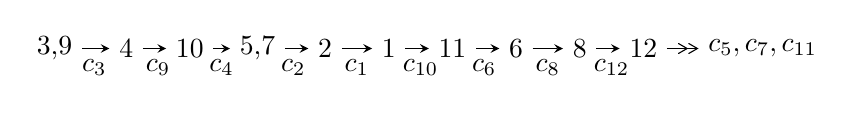
\begin{tikzpicture}[x=23pt, y=7pt]
	% node
	\node (A0) at (-1/8, 0) {3,9};
	\node (A1) at (1, 0) {4};
	\node (A2) at (2, 0) {10};
	\node (A3) at (49/16, 0) {5,7};
	\node (A4) at (33/8, 0) {2};
	\node (A5) at (41/8, 0) {1};
	\node (A6) at (49/8, 0) {11};
	\node (A7) at (57/8, 0) {6};
	\node (A8) at (65/8, 0) {8};
	\node (A9) at (73/8, 0) {12};
	\node (C1) at (1/2, -1) {$c_{3}$};
	\node (C2) at (3/2, -1) {$c_{9}$};
	\node (C3) at (5/2, -1) {$c_{4}$};
	\node (C4) at (29/8, -1) {$c_{2}$};
	\node (C5) at (37/8, -1) {$c_{1}$};
	\node (C6) at (45/8, -1) {$c_{10}$};
	\node (C7) at (53/8, -1) {$c_{6}$};
	\node (C8) at (61/8, -1) {$c_{8}$};
	\node (C9) at (69/8, -1) {$c_{12}$};
	\node (A10) at (11, 0) {$c_{5},c_{7},c_{11}$};

	% edge
	\draw[->,>=stealth]	
	(A0) edge (A1) (A1) edge (A2) (A2) edge (A3) (A3) edge (A4) (A4) edge (A5) (A5) edge (A6) (A6) edge (A7) (A7) edge (A8) (A8) edge (A9) ;
	\draw[->>,>={angle 60}]	
	(A9) edge (A10);
\end{tikzpicture} \\ 

\end{tabular} \\

\footnotetext{
The image of knot diagram is generated by the software ``\textbf{Draw programme}" developed by Andrew Bartholomew(\url{http://www.layer8.co.uk/maths/draw/index.htm\#Running-draw}), where we modified some parts for our purpose(\url{https://github.com/CATsTAILs/LinksPainter}).
}\phantom \\ \newline 
\centering \textbf{Ideals for irreducible components\footnotemark of $X_{\text{par}}$} 
 
\begin{align*}
I^u_{1}&=\langle 
2.31307\times10^{165} u^{121}+5.38073\times10^{164} u^{120}+\cdots+4.90444\times10^{165} b-6.70880\times10^{165},\\
\phantom{I^u_{1}}&\phantom{= \langle  }-3.23704\times10^{165} u^{121}-2.41638\times10^{165} u^{120}+\cdots+4.90444\times10^{165} a+1.05285\times10^{166},\\
\phantom{I^u_{1}}&\phantom{= \langle  }u^{122}- u^{121}+\cdots+14 u-1\rangle \\
I^u_{2}&=\langle 
u^{20}-8 u^{18}+\cdots+b-1,\;2 u^{20}- u^{19}+\cdots+a-7,\;u^{21}-10 u^{19}+\cdots-7 u+1\rangle \\
\\
\end{align*}
\raggedright * 2 irreducible components of $\dim_{\mathbb{C}}=0$, with total 143 representations.\\
\footnotetext{All coefficients of polynomials are rational numbers. But the coefficients are sometimes approximated in decimal forms when there is not enough margin.}
\newpage
\renewcommand{\arraystretch}{1}
\centering \section*{I. $I^u_{1}= \langle 2.31\times10^{165} u^{121}+5.38\times10^{164} u^{120}+\cdots+4.90\times10^{165} b-6.71\times10^{165},\;-3.24\times10^{165} u^{121}-2.42\times10^{165} u^{120}+\cdots+4.90\times10^{165} a+1.05\times10^{166},\;u^{122}- u^{121}+\cdots+14 u-1 \rangle$}
\flushleft \textbf{(i) Arc colorings}\\
\begin{tabular}{m{7pt} m{180pt} m{7pt} m{180pt} }
\flushright $a_{3}=$&$\begin{pmatrix}1\\0\end{pmatrix}$ \\
\flushright $a_{9}=$&$\begin{pmatrix}0\\u\end{pmatrix}$ \\
\flushright $a_{4}=$&$\begin{pmatrix}1\\u^2\end{pmatrix}$ \\
\flushright $a_{10}=$&$\begin{pmatrix}- u\\- u^3+u\end{pmatrix}$ \\
\flushright $a_{5}=$&$\begin{pmatrix}- u^2+1\\- u^4+2 u^2\end{pmatrix}$ \\
\flushright $a_{7}=$&$\begin{pmatrix}0.660022 u^{121}+0.492694 u^{120}+\cdots-53.1593 u-2.14673\\-0.471629 u^{121}-0.109712 u^{120}+\cdots-3.50950 u+1.36790\end{pmatrix}$ \\
\flushright $a_{2}=$&$\begin{pmatrix}-0.743016 u^{121}-0.880764 u^{120}+\cdots+5.83100 u+8.73557\\0.0920455 u^{121}+0.774925 u^{120}+\cdots+13.2435 u-1.69094\end{pmatrix}$ \\
\flushright $a_{1}=$&$\begin{pmatrix}-0.650971 u^{121}-0.105839 u^{120}+\cdots+19.0745 u+7.04462\\0.0920455 u^{121}+0.774925 u^{120}+\cdots+13.2435 u-1.69094\end{pmatrix}$ \\
\flushright $a_{11}=$&$\begin{pmatrix}2.30111 u^{121}+0.0727856 u^{120}+\cdots-140.337 u+6.38639\\-0.887005 u^{121}+0.100156 u^{120}+\cdots+24.1947 u-0.623252\end{pmatrix}$ \\
\flushright $a_{6}=$&$\begin{pmatrix}-0.308103 u^{121}-0.0346067 u^{120}+\cdots-134.651 u+11.8650\\-0.749272 u^{121}+1.31527 u^{120}+\cdots+18.1101 u-0.0215096\end{pmatrix}$ \\
\flushright $a_{8}=$&$\begin{pmatrix}u^5-2 u^3+u\\u^7-3 u^5+2 u^3+u\end{pmatrix}$ \\
\flushright $a_{12}=$&$\begin{pmatrix}-1.05192 u^{121}-0.921213 u^{120}+\cdots+24.4218 u+6.68467\\0.194588 u^{121}+0.843786 u^{120}+\cdots+12.8019 u-1.63077\end{pmatrix}$\\&\end{tabular}
\flushleft \textbf{(ii) Obstruction class $= -1$}\\~\\
\flushleft \textbf{(iii) Cusp Shapes $= 0.935769 u^{121}-0.911728 u^{120}+\cdots-17.5892 u-7.15303$}\\~\\
\newpage\renewcommand{\arraystretch}{1}
\flushleft \textbf{(iv) u-Polynomials at the component}\newline \\
\begin{tabular}{m{50pt}|m{274pt}}
Crossings & \hspace{64pt}u-Polynomials at each crossing \\
\hline $$\begin{aligned}c_{1}\end{aligned}$$&$\begin{aligned}
&u^{122}+46 u^{121}+\cdots+56468 u+841
\end{aligned}$\\
\hline $$\begin{aligned}c_{2},c_{6}\end{aligned}$$&$\begin{aligned}
&u^{122}-2 u^{121}+\cdots+18 u+29
\end{aligned}$\\
\hline $$\begin{aligned}c_{3},c_{4},c_{9}\end{aligned}$$&$\begin{aligned}
&u^{122}- u^{121}+\cdots+14 u-1
\end{aligned}$\\
\hline $$\begin{aligned}c_{5},c_{11}\end{aligned}$$&$\begin{aligned}
&u^{122}- u^{121}+\cdots+35 u-1
\end{aligned}$\\
\hline $$\begin{aligned}c_{7}\end{aligned}$$&$\begin{aligned}
&u^{122}+8 u^{121}+\cdots-298520 u-40207
\end{aligned}$\\
\hline $$\begin{aligned}c_{8}\end{aligned}$$&$\begin{aligned}
&u^{122}+3 u^{121}+\cdots-10052 u+949
\end{aligned}$\\
\hline $$\begin{aligned}c_{10}\end{aligned}$$&$\begin{aligned}
&u^{122}-20 u^{121}+\cdots-18800 u+1457
\end{aligned}$\\
\hline $$\begin{aligned}c_{12}\end{aligned}$$&$\begin{aligned}
&u^{122}-2 u^{121}+\cdots-1232502 u-100871
\end{aligned}$\\
\hline
\end{tabular}\\~\\
\newpage\renewcommand{\arraystretch}{1}
\flushleft \textbf{(v) Riley Polynomials at the component}\newline \\
\begin{tabular}{m{50pt}|m{274pt}}
Crossings & \hspace{64pt}Riley Polynomials at each crossing \\
\hline $$\begin{aligned}c_{1}\end{aligned}$$&$\begin{aligned}
&y^{122}+70 y^{121}+\cdots-130799392 y+707281
\end{aligned}$\\
\hline $$\begin{aligned}c_{2},c_{6}\end{aligned}$$&$\begin{aligned}
&y^{122}-46 y^{121}+\cdots-56468 y+841
\end{aligned}$\\
\hline $$\begin{aligned}c_{3},c_{4},c_{9}\end{aligned}$$&$\begin{aligned}
&y^{122}-105 y^{121}+\cdots+116 y+1
\end{aligned}$\\
\hline $$\begin{aligned}c_{5},c_{11}\end{aligned}$$&$\begin{aligned}
&y^{122}+99 y^{121}+\cdots+173 y+1
\end{aligned}$\\
\hline $$\begin{aligned}c_{7}\end{aligned}$$&$\begin{aligned}
&y^{122}+34 y^{121}+\cdots+9443298764 y+1616602849
\end{aligned}$\\
\hline $$\begin{aligned}c_{8}\end{aligned}$$&$\begin{aligned}
&y^{122}+59 y^{121}+\cdots+89191938 y+900601
\end{aligned}$\\
\hline $$\begin{aligned}c_{10}\end{aligned}$$&$\begin{aligned}
&y^{122}+18 y^{121}+\cdots-67920452 y+2122849
\end{aligned}$\\
\hline $$\begin{aligned}c_{12}\end{aligned}$$&$\begin{aligned}
&y^{122}+30 y^{121}+\cdots+188566629184 y+10174958641
\end{aligned}$\\
\hline
\end{tabular}\\~\\
\newpage\flushleft \textbf{(vi) Complex Volumes and Cusp Shapes}
$$\begin{array}{c|c|c}  
\text{Solutions to }I^u_{1}& \I (\text{vol} + \sqrt{-1}CS) & \text{Cusp shape}\\
 \hline 
\begin{aligned}
u &= -0.234555 + 0.988031 I \\
a &= \phantom{-}0.92156 + 1.12342 I \\
b &= -0.872223 - 0.630867 I\end{aligned}
 & \phantom{-}5.72527 - 1.28507 I & \phantom{-0.000000 } 0 \\ \hline\begin{aligned}
u &= -0.234555 - 0.988031 I \\
a &= \phantom{-}0.92156 - 1.12342 I \\
b &= -0.872223 + 0.630867 I\end{aligned}
 & \phantom{-}5.72527 + 1.28507 I & \phantom{-0.000000 } 0 \\ \hline\begin{aligned}
u &= \phantom{-}0.760590 + 0.674896 I \\
a &= -0.316027 + 0.926892 I \\
b &= \phantom{-}0.686502 - 0.641692 I\end{aligned}
 & \phantom{-}4.42128 - 1.94594 I & \phantom{-0.000000 } 0 \\ \hline\begin{aligned}
u &= \phantom{-}0.760590 - 0.674896 I \\
a &= -0.316027 - 0.926892 I \\
b &= \phantom{-}0.686502 + 0.641692 I\end{aligned}
 & \phantom{-}4.42128 + 1.94594 I & \phantom{-0.000000 } 0 \\ \hline\begin{aligned}
u &= \phantom{-}0.322630 + 0.970146 I \\
a &= \phantom{-}0.10806 + 1.82890 I \\
b &= -0.828609 - 0.630177 I\end{aligned}
 & \phantom{-}5.86251 - 3.65151 I & \phantom{-0.000000 } 0 \\ \hline\begin{aligned}
u &= \phantom{-}0.322630 - 0.970146 I \\
a &= \phantom{-}0.10806 - 1.82890 I \\
b &= -0.828609 + 0.630177 I\end{aligned}
 & \phantom{-}5.86251 + 3.65151 I & \phantom{-0.000000 } 0 \\ \hline\begin{aligned}
u &= -0.214504 + 0.861105 I \\
a &= \phantom{-}0.44544 - 2.29325 I \\
b &= -1.099800 + 0.728566 I\end{aligned}
 & \phantom{-}6.9239 + 14.0853 I & \phantom{-0.000000 } 0 \\ \hline\begin{aligned}
u &= -0.214504 - 0.861105 I \\
a &= \phantom{-}0.44544 + 2.29325 I \\
b &= -1.099800 - 0.728566 I\end{aligned}
 & \phantom{-}6.9239 - 14.0853 I & \phantom{-0.000000 } 0 \\ \hline\begin{aligned}
u &= -1.001190 + 0.502220 I \\
a &= -0.467524 - 0.781643 I \\
b &= \phantom{-}1.068540 + 0.711550 I\end{aligned}
 & \phantom{-}4.50697 - 9.26659 I & \phantom{-0.000000 } 0 \\ \hline\begin{aligned}
u &= -1.001190 - 0.502220 I \\
a &= -0.467524 + 0.781643 I \\
b &= \phantom{-}1.068540 - 0.711550 I\end{aligned}
 & \phantom{-}4.50697 + 9.26659 I & \phantom{-0.000000 } 0\\
 \hline 
 \end{array}$$\newpage$$\begin{array}{c|c|c}  
\text{Solutions to }I^u_{1}& \I (\text{vol} + \sqrt{-1}CS) & \text{Cusp shape}\\
 \hline 
\begin{aligned}
u &= \phantom{-}1.030580 + 0.445182 I \\
a &= \phantom{-}0.13785 - 1.45127 I \\
b &= \phantom{-}0.610203 + 0.880621 I\end{aligned}
 & \phantom{-}5.91876 + 3.36739 I & \phantom{-0.000000 } 0 \\ \hline\begin{aligned}
u &= \phantom{-}1.030580 - 0.445182 I \\
a &= \phantom{-}0.13785 + 1.45127 I \\
b &= \phantom{-}0.610203 - 0.880621 I\end{aligned}
 & \phantom{-}5.91876 - 3.36739 I & \phantom{-0.000000 } 0 \\ \hline\begin{aligned}
u &= -1.107230 + 0.202197 I \\
a &= \phantom{-}0.353996 - 0.891172 I \\
b &= -0.690022 + 0.709843 I\end{aligned}
 & \phantom{-}0.251889 + 0.777032 I & \phantom{-0.000000 } 0 \\ \hline\begin{aligned}
u &= -1.107230 - 0.202197 I \\
a &= \phantom{-}0.353996 + 0.891172 I \\
b &= -0.690022 - 0.709843 I\end{aligned}
 & \phantom{-}0.251889 - 0.777032 I & \phantom{-0.000000 } 0 \\ \hline\begin{aligned}
u &= -0.915379 + 0.675967 I \\
a &= \phantom{-}0.02342 + 1.50127 I \\
b &= \phantom{-}0.959430 - 0.636264 I\end{aligned}
 & \phantom{-}3.60956 + 6.96571 I & \phantom{-0.000000 } 0 \\ \hline\begin{aligned}
u &= -0.915379 - 0.675967 I \\
a &= \phantom{-}0.02342 - 1.50127 I \\
b &= \phantom{-}0.959430 + 0.636264 I\end{aligned}
 & \phantom{-}3.60956 - 6.96571 I & \phantom{-0.000000 } 0 \\ \hline\begin{aligned}
u &= \phantom{-}0.186110 + 0.839501 I \\
a &= \phantom{-}1.18588 - 1.51108 I \\
b &= -0.588144 + 0.942203 I\end{aligned}
 & \phantom{-}8.51107 - 7.96464 I & \phantom{-0.000000 } 0 \\ \hline\begin{aligned}
u &= \phantom{-}0.186110 - 0.839501 I \\
a &= \phantom{-}1.18588 + 1.51108 I \\
b &= -0.588144 - 0.942203 I\end{aligned}
 & \phantom{-}8.51107 + 7.96464 I & \phantom{-0.000000 } 0 \\ \hline\begin{aligned}
u &= \phantom{-}1.137060 + 0.083755 I \\
a &= -0.340810 - 1.362340 I \\
b &= -0.970198 + 0.697036 I\end{aligned}
 & -0.52167 + 4.61172 I & \phantom{-0.000000 } 0 \\ \hline\begin{aligned}
u &= \phantom{-}1.137060 - 0.083755 I \\
a &= -0.340810 + 1.362340 I \\
b &= -0.970198 - 0.697036 I\end{aligned}
 & -0.52167 - 4.61172 I & \phantom{-0.000000 } 0\\
 \hline 
 \end{array}$$\newpage$$\begin{array}{c|c|c}  
\text{Solutions to }I^u_{1}& \I (\text{vol} + \sqrt{-1}CS) & \text{Cusp shape}\\
 \hline 
\begin{aligned}
u &= -1.113200 + 0.350252 I \\
a &= \phantom{-}0.316835 + 0.134474 I \\
b &= -0.792717 + 0.032554 I\end{aligned}
 & -0.01080 + 2.42638 I & \phantom{-0.000000 } 0 \\ \hline\begin{aligned}
u &= -1.113200 - 0.350252 I \\
a &= \phantom{-}0.316835 - 0.134474 I \\
b &= -0.792717 - 0.032554 I\end{aligned}
 & -0.01080 - 2.42638 I & \phantom{-0.000000 } 0 \\ \hline\begin{aligned}
u &= \phantom{-}1.153350 + 0.243735 I \\
a &= -0.366981 + 1.183590 I \\
b &= -0.801289 - 0.738462 I\end{aligned}
 & -0.16714 - 4.78859 I & \phantom{-0.000000 } 0 \\ \hline\begin{aligned}
u &= \phantom{-}1.153350 - 0.243735 I \\
a &= -0.366981 - 1.183590 I \\
b &= -0.801289 + 0.738462 I\end{aligned}
 & -0.16714 + 4.78859 I & \phantom{-0.000000 } 0 \\ \hline\begin{aligned}
u &= -0.099249 + 0.797317 I \\
a &= -0.716625 + 0.713497 I \\
b &= \phantom{-}0.620262 - 0.047717 I\end{aligned}
 & \phantom{-}3.11143 + 1.77129 I & -12.00000 - 3.74305 I \\ \hline\begin{aligned}
u &= -0.099249 - 0.797317 I \\
a &= -0.716625 - 0.713497 I \\
b &= \phantom{-}0.620262 + 0.047717 I\end{aligned}
 & \phantom{-}3.11143 - 1.77129 I & -12.00000 + 3.74305 I \\ \hline\begin{aligned}
u &= -0.724566 + 0.333200 I \\
a &= \phantom{-}0.084913 - 0.920619 I \\
b &= -1.117180 - 0.110982 I\end{aligned}
 & -0.93866 - 2.49661 I & -12.00000 + 2.74029 I \\ \hline\begin{aligned}
u &= -0.724566 - 0.333200 I \\
a &= \phantom{-}0.084913 + 0.920619 I \\
b &= -1.117180 + 0.110982 I\end{aligned}
 & -0.93866 + 2.49661 I & -12.00000 - 2.74029 I \\ \hline\begin{aligned}
u &= -1.218930 + 0.045329 I \\
a &= \phantom{-}0.380004 + 0.484744 I \\
b &= -0.786560 - 0.829293 I\end{aligned}
 & -0.047384 - 0.970006 I & \phantom{-0.000000 } 0 \\ \hline\begin{aligned}
u &= -1.218930 - 0.045329 I \\
a &= \phantom{-}0.380004 - 0.484744 I \\
b &= -0.786560 + 0.829293 I\end{aligned}
 & -0.047384 + 0.970006 I & \phantom{-0.000000 } 0\\
 \hline 
 \end{array}$$\newpage$$\begin{array}{c|c|c}  
\text{Solutions to }I^u_{1}& \I (\text{vol} + \sqrt{-1}CS) & \text{Cusp shape}\\
 \hline 
\begin{aligned}
u &= \phantom{-}0.744074 + 0.182009 I \\
a &= -0.429229 - 0.732669 I \\
b &= -0.947133 + 0.634087 I\end{aligned}
 & -0.40422 + 4.44938 I & -14.0673 - 4.9668 I \\ \hline\begin{aligned}
u &= \phantom{-}0.744074 - 0.182009 I \\
a &= -0.429229 + 0.732669 I \\
b &= -0.947133 - 0.634087 I\end{aligned}
 & -0.40422 - 4.44938 I & -14.0673 + 4.9668 I \\ \hline\begin{aligned}
u &= \phantom{-}0.189284 + 0.736058 I \\
a &= \phantom{-}0.04393 - 2.54745 I \\
b &= \phantom{-}1.023300 + 0.644874 I\end{aligned}
 & \phantom{-}1.77068 - 8.04690 I & -9.57286 + 9.37019 I \\ \hline\begin{aligned}
u &= \phantom{-}0.189284 - 0.736058 I \\
a &= \phantom{-}0.04393 + 2.54745 I \\
b &= \phantom{-}1.023300 - 0.644874 I\end{aligned}
 & \phantom{-}1.77068 + 8.04690 I & -9.57286 - 9.37019 I \\ \hline\begin{aligned}
u &= -0.221698 + 0.720542 I \\
a &= -0.770295 + 0.907435 I \\
b &= \phantom{-}1.281360 - 0.189413 I\end{aligned}
 & \phantom{-}0.84791 + 6.25400 I & -11.2890 - 8.6710 I \\ \hline\begin{aligned}
u &= -0.221698 - 0.720542 I \\
a &= -0.770295 - 0.907435 I \\
b &= \phantom{-}1.281360 + 0.189413 I\end{aligned}
 & \phantom{-}0.84791 - 6.25400 I & -11.2890 + 8.6710 I \\ \hline\begin{aligned}
u &= -0.140582 + 0.739623 I \\
a &= -1.39916 - 0.87483 I \\
b &= \phantom{-}0.574494 + 0.702034 I\end{aligned}
 & \phantom{-}3.07037 + 2.84110 I & -7.29913 - 4.46443 I \\ \hline\begin{aligned}
u &= -0.140582 - 0.739623 I \\
a &= -1.39916 + 0.87483 I \\
b &= \phantom{-}0.574494 - 0.702034 I\end{aligned}
 & \phantom{-}3.07037 - 2.84110 I & -7.29913 + 4.46443 I \\ \hline\begin{aligned}
u &= -1.243150 + 0.100960 I \\
a &= -0.738286 - 0.774980 I \\
b &= -1.204120 - 0.528067 I\end{aligned}
 & -1.17292 - 3.59071 I & \phantom{-0.000000 } 0 \\ \hline\begin{aligned}
u &= -1.243150 - 0.100960 I \\
a &= -0.738286 + 0.774980 I \\
b &= -1.204120 + 0.528067 I\end{aligned}
 & -1.17292 + 3.59071 I & \phantom{-0.000000 } 0\\
 \hline 
 \end{array}$$\newpage$$\begin{array}{c|c|c}  
\text{Solutions to }I^u_{1}& \I (\text{vol} + \sqrt{-1}CS) & \text{Cusp shape}\\
 \hline 
\begin{aligned}
u &= \phantom{-}0.074658 + 0.742254 I \\
a &= -0.81283 + 1.26950 I \\
b &= \phantom{-}0.587696 - 0.654971 I\end{aligned}
 & \phantom{-}3.04979 + 1.07688 I & -7.24896 - 3.00156 I \\ \hline\begin{aligned}
u &= \phantom{-}0.074658 - 0.742254 I \\
a &= -0.81283 - 1.26950 I \\
b &= \phantom{-}0.587696 + 0.654971 I\end{aligned}
 & \phantom{-}3.04979 - 1.07688 I & -7.24896 + 3.00156 I \\ \hline\begin{aligned}
u &= -0.228245 + 0.709352 I \\
a &= -0.37252 + 2.01880 I \\
b &= \phantom{-}1.003610 - 0.619740 I\end{aligned}
 & \phantom{-}1.85617 + 3.92199 I & -9.76878 - 2.82515 I \\ \hline\begin{aligned}
u &= -0.228245 - 0.709352 I \\
a &= -0.37252 - 2.01880 I \\
b &= \phantom{-}1.003610 + 0.619740 I\end{aligned}
 & \phantom{-}1.85617 - 3.92199 I & -9.76878 + 2.82515 I \\ \hline\begin{aligned}
u &= \phantom{-}1.226380 + 0.265835 I \\
a &= -1.177270 + 0.321168 I \\
b &= \phantom{-}0.321693 - 1.143740 I\end{aligned}
 & \phantom{-}3.59136 - 1.45213 I & \phantom{-0.000000 } 0 \\ \hline\begin{aligned}
u &= \phantom{-}1.226380 - 0.265835 I \\
a &= -1.177270 - 0.321168 I \\
b &= \phantom{-}0.321693 + 1.143740 I\end{aligned}
 & \phantom{-}3.59136 + 1.45213 I & \phantom{-0.000000 } 0 \\ \hline\begin{aligned}
u &= \phantom{-}1.249820 + 0.142486 I \\
a &= -2.82499 + 0.56538 I \\
b &= -0.755633 + 0.350064 I\end{aligned}
 & \phantom{-}0.762504 - 0.559043 I & \phantom{-0.000000 } 0 \\ \hline\begin{aligned}
u &= \phantom{-}1.249820 - 0.142486 I \\
a &= -2.82499 - 0.56538 I \\
b &= -0.755633 - 0.350064 I\end{aligned}
 & \phantom{-}0.762504 + 0.559043 I & \phantom{-0.000000 } 0 \\ \hline\begin{aligned}
u &= -0.017426 + 0.740999 I \\
a &= \phantom{-}2.34826 - 1.92460 I \\
b &= -0.869803 + 0.657397 I\end{aligned}
 & \phantom{-}6.22351 + 4.56633 I & -3.73730 - 6.98496 I \\ \hline\begin{aligned}
u &= -0.017426 - 0.740999 I \\
a &= \phantom{-}2.34826 + 1.92460 I \\
b &= -0.869803 - 0.657397 I\end{aligned}
 & \phantom{-}6.22351 - 4.56633 I & -3.73730 + 6.98496 I\\
 \hline 
 \end{array}$$\newpage$$\begin{array}{c|c|c}  
\text{Solutions to }I^u_{1}& \I (\text{vol} + \sqrt{-1}CS) & \text{Cusp shape}\\
 \hline 
\begin{aligned}
u &= \phantom{-}1.26617\phantom{ +0.000000I} \\
a &= \phantom{-}1.31692\phantom{ +0.000000I} \\
b &= -0.525476\phantom{ +0.000000I}\end{aligned}
 & -6.18263\phantom{ +0.000000I} & \phantom{-0.000000 } 0 \\ \hline\begin{aligned}
u &= \phantom{-}0.058524 + 0.715391 I \\
a &= \phantom{-}0.75668 + 2.16588 I \\
b &= -0.464647 - 1.129910 I\end{aligned}
 & \phantom{-}7.14471 - 2.10096 I & \phantom{-}1.17722 + 2.65730 I \\ \hline\begin{aligned}
u &= \phantom{-}0.058524 - 0.715391 I \\
a &= \phantom{-}0.75668 - 2.16588 I \\
b &= -0.464647 + 1.129910 I\end{aligned}
 & \phantom{-}7.14471 + 2.10096 I & \phantom{-}1.17722 - 2.65730 I \\ \hline\begin{aligned}
u &= -1.251400 + 0.304571 I \\
a &= -1.85642 - 0.08555 I \\
b &= \phantom{-}0.843838 + 0.614687 I\end{aligned}
 & \phantom{-}2.41412 - 0.78698 I & \phantom{-0.000000 } 0 \\ \hline\begin{aligned}
u &= -1.251400 - 0.304571 I \\
a &= -1.85642 + 0.08555 I \\
b &= \phantom{-}0.843838 - 0.614687 I\end{aligned}
 & \phantom{-}2.41412 + 0.78698 I & \phantom{-0.000000 } 0 \\ \hline\begin{aligned}
u &= \phantom{-}1.260920 + 0.268599 I \\
a &= -0.645813 + 0.337662 I \\
b &= \phantom{-}1.12107 - 0.86570 I\end{aligned}
 & \phantom{-}1.21395 + 1.35004 I & \phantom{-0.000000 } 0 \\ \hline\begin{aligned}
u &= \phantom{-}1.260920 - 0.268599 I \\
a &= -0.645813 - 0.337662 I \\
b &= \phantom{-}1.12107 + 0.86570 I\end{aligned}
 & \phantom{-}1.21395 - 1.35004 I & \phantom{-0.000000 } 0 \\ \hline\begin{aligned}
u &= -1.274760 + 0.275843 I \\
a &= -0.89496 - 1.60223 I \\
b &= \phantom{-}0.828740 + 0.712699 I\end{aligned}
 & \phantom{-}2.37321 + 2.95488 I & \phantom{-0.000000 } 0 \\ \hline\begin{aligned}
u &= -1.274760 - 0.275843 I \\
a &= -0.89496 + 1.60223 I \\
b &= \phantom{-}0.828740 - 0.712699 I\end{aligned}
 & \phantom{-}2.37321 - 2.95488 I & \phantom{-0.000000 } 0 \\ \hline\begin{aligned}
u &= \phantom{-}0.024434 + 0.693745 I \\
a &= \phantom{-}1.18639 + 2.36959 I \\
b &= -1.17157 - 0.81956 I\end{aligned}
 & \phantom{-}5.03237 - 4.82256 I & -4.82716 + 7.18113 I\\
 \hline 
 \end{array}$$\newpage$$\begin{array}{c|c|c}  
\text{Solutions to }I^u_{1}& \I (\text{vol} + \sqrt{-1}CS) & \text{Cusp shape}\\
 \hline 
\begin{aligned}
u &= \phantom{-}0.024434 - 0.693745 I \\
a &= \phantom{-}1.18639 - 2.36959 I \\
b &= -1.17157 + 0.81956 I\end{aligned}
 & \phantom{-}5.03237 + 4.82256 I & -4.82716 - 7.18113 I \\ \hline\begin{aligned}
u &= -0.001317 + 0.691952 I \\
a &= \phantom{-}0.85529 - 3.52300 I \\
b &= -0.835681 + 0.659362 I\end{aligned}
 & \phantom{-}6.32991 + 0.54399 I & -3.29943 - 0.17721 I \\ \hline\begin{aligned}
u &= -0.001317 - 0.691952 I \\
a &= \phantom{-}0.85529 + 3.52300 I \\
b &= -0.835681 - 0.659362 I\end{aligned}
 & \phantom{-}6.32991 - 0.54399 I & -3.29943 + 0.17721 I \\ \hline\begin{aligned}
u &= \phantom{-}1.280480 + 0.271970 I \\
a &= \phantom{-}1.44341 - 3.07056 I \\
b &= \phantom{-}0.866416 + 0.606863 I\end{aligned}
 & \phantom{-}2.34431 - 4.02005 I & \phantom{-0.000000 } 0 \\ \hline\begin{aligned}
u &= \phantom{-}1.280480 - 0.271970 I \\
a &= \phantom{-}1.44341 + 3.07056 I \\
b &= \phantom{-}0.866416 - 0.606863 I\end{aligned}
 & \phantom{-}2.34431 + 4.02005 I & \phantom{-0.000000 } 0 \\ \hline\begin{aligned}
u &= \phantom{-}1.278930 + 0.304729 I \\
a &= -0.58243 - 2.07900 I \\
b &= \phantom{-}0.885814 + 0.693929 I\end{aligned}
 & \phantom{-}2.19424 - 8.34091 I & \phantom{-0.000000 } 0 \\ \hline\begin{aligned}
u &= \phantom{-}1.278930 - 0.304729 I \\
a &= -0.58243 + 2.07900 I \\
b &= \phantom{-}0.885814 - 0.693929 I\end{aligned}
 & \phantom{-}2.19424 + 8.34091 I & \phantom{-0.000000 } 0 \\ \hline\begin{aligned}
u &= -1.291330 + 0.278909 I \\
a &= \phantom{-}1.05610 + 2.01348 I \\
b &= \phantom{-}1.22927 - 0.79308 I\end{aligned}
 & \phantom{-}0.92503 + 8.33903 I & \phantom{-0.000000 } 0 \\ \hline\begin{aligned}
u &= -1.291330 - 0.278909 I \\
a &= \phantom{-}1.05610 - 2.01348 I \\
b &= \phantom{-}1.22927 + 0.79308 I\end{aligned}
 & \phantom{-}0.92503 - 8.33903 I & \phantom{-0.000000 } 0 \\ \hline\begin{aligned}
u &= -0.642168 + 0.198301 I \\
a &= \phantom{-}0.265917 + 0.199592 I \\
b &= -0.798044 - 0.574498 I\end{aligned}
 & \phantom{-}0.088768 - 0.449411 I & -13.05283 - 1.45306 I\\
 \hline 
 \end{array}$$\newpage$$\begin{array}{c|c|c}  
\text{Solutions to }I^u_{1}& \I (\text{vol} + \sqrt{-1}CS) & \text{Cusp shape}\\
 \hline 
\begin{aligned}
u &= -0.642168 - 0.198301 I \\
a &= \phantom{-}0.265917 - 0.199592 I \\
b &= -0.798044 + 0.574498 I\end{aligned}
 & \phantom{-}0.088768 + 0.449411 I & -13.05283 + 1.45306 I \\ \hline\begin{aligned}
u &= \phantom{-}1.327070 + 0.137247 I \\
a &= \phantom{-}0.857852 - 0.085963 I \\
b &= \phantom{-}1.006020 - 0.206204 I\end{aligned}
 & -5.49406 - 0.39217 I & \phantom{-0.000000 } 0 \\ \hline\begin{aligned}
u &= \phantom{-}1.327070 - 0.137247 I \\
a &= \phantom{-}0.857852 + 0.085963 I \\
b &= \phantom{-}1.006020 + 0.206204 I\end{aligned}
 & -5.49406 + 0.39217 I & \phantom{-0.000000 } 0 \\ \hline\begin{aligned}
u &= -1.304730 + 0.295079 I \\
a &= \phantom{-}0.591703 + 1.234260 I \\
b &= \phantom{-}0.566057 - 1.150080 I\end{aligned}
 & \phantom{-}2.87894 + 5.75928 I & \phantom{-0.000000 } 0 \\ \hline\begin{aligned}
u &= -1.304730 - 0.295079 I \\
a &= \phantom{-}0.591703 - 1.234260 I \\
b &= \phantom{-}0.566057 + 1.150080 I\end{aligned}
 & \phantom{-}2.87894 - 5.75928 I & \phantom{-0.000000 } 0 \\ \hline\begin{aligned}
u &= -1.307990 + 0.288818 I \\
a &= \phantom{-}0.545872 + 0.387828 I \\
b &= -0.375293 - 0.698799 I\end{aligned}
 & -1.24382 + 2.63179 I & \phantom{-0.000000 } 0 \\ \hline\begin{aligned}
u &= -1.307990 - 0.288818 I \\
a &= \phantom{-}0.545872 - 0.387828 I \\
b &= -0.375293 + 0.698799 I\end{aligned}
 & -1.24382 - 2.63179 I & \phantom{-0.000000 } 0 \\ \hline\begin{aligned}
u &= \phantom{-}0.293912 + 0.579535 I \\
a &= \phantom{-}0.55904 + 1.34017 I \\
b &= \phantom{-}0.431291 - 0.009036 I\end{aligned}
 & \phantom{-}3.65162 - 1.53173 I & -11.67260 + 4.52649 I \\ \hline\begin{aligned}
u &= \phantom{-}0.293912 - 0.579535 I \\
a &= \phantom{-}0.55904 - 1.34017 I \\
b &= \phantom{-}0.431291 + 0.009036 I\end{aligned}
 & \phantom{-}3.65162 + 1.53173 I & -11.67260 - 4.52649 I \\ \hline\begin{aligned}
u &= \phantom{-}1.356340 + 0.002377 I \\
a &= \phantom{-}0.509631 - 0.034649 I \\
b &= \phantom{-}0.453652 - 0.267196 I\end{aligned}
 & -5.69404 - 0.04855 I & \phantom{-0.000000 } 0\\
 \hline 
 \end{array}$$\newpage$$\begin{array}{c|c|c}  
\text{Solutions to }I^u_{1}& \I (\text{vol} + \sqrt{-1}CS) & \text{Cusp shape}\\
 \hline 
\begin{aligned}
u &= \phantom{-}1.356340 - 0.002377 I \\
a &= \phantom{-}0.509631 + 0.034649 I \\
b &= \phantom{-}0.453652 + 0.267196 I\end{aligned}
 & -5.69404 + 0.04855 I & \phantom{-0.000000 } 0 \\ \hline\begin{aligned}
u &= -1.345300 + 0.250381 I \\
a &= \phantom{-}1.28141 + 0.84426 I \\
b &= \phantom{-}1.143410 + 0.068518 I\end{aligned}
 & -6.80581 + 4.92030 I & \phantom{-0.000000 } 0 \\ \hline\begin{aligned}
u &= -1.345300 - 0.250381 I \\
a &= \phantom{-}1.28141 - 0.84426 I \\
b &= \phantom{-}1.143410 - 0.068518 I\end{aligned}
 & -6.80581 - 4.92030 I & \phantom{-0.000000 } 0 \\ \hline\begin{aligned}
u &= \phantom{-}1.328260 + 0.336809 I \\
a &= -0.030301 + 0.823161 I \\
b &= -0.522814 - 0.039632 I\end{aligned}
 & -1.36278 - 5.84823 I & \phantom{-0.000000 } 0 \\ \hline\begin{aligned}
u &= \phantom{-}1.328260 - 0.336809 I \\
a &= -0.030301 - 0.823161 I \\
b &= -0.522814 + 0.039632 I\end{aligned}
 & -1.36278 + 5.84823 I & \phantom{-0.000000 } 0 \\ \hline\begin{aligned}
u &= -1.372790 + 0.115216 I \\
a &= -1.61595 - 1.42202 I \\
b &= -1.029850 + 0.272400 I\end{aligned}
 & -8.54849 + 2.02896 I & \phantom{-0.000000 } 0 \\ \hline\begin{aligned}
u &= -1.372790 - 0.115216 I \\
a &= -1.61595 + 1.42202 I \\
b &= -1.029850 - 0.272400 I\end{aligned}
 & -8.54849 - 2.02896 I & \phantom{-0.000000 } 0 \\ \hline\begin{aligned}
u &= \phantom{-}1.346710 + 0.311323 I \\
a &= \phantom{-}0.917348 + 0.125384 I \\
b &= -0.508217 + 0.711957 I\end{aligned}
 & -1.61438 - 6.65221 I & \phantom{-0.000000 } 0 \\ \hline\begin{aligned}
u &= \phantom{-}1.346710 - 0.311323 I \\
a &= \phantom{-}0.917348 - 0.125384 I \\
b &= -0.508217 - 0.711957 I\end{aligned}
 & -1.61438 + 6.65221 I & \phantom{-0.000000 } 0 \\ \hline\begin{aligned}
u &= \phantom{-}0.145021 + 0.596292 I \\
a &= \phantom{-}0.025912 + 0.660063 I \\
b &= -1.070710 + 0.023694 I\end{aligned}
 & -2.09996 - 1.78711 I & -13.9383 + 4.1525 I\\
 \hline 
 \end{array}$$\newpage$$\begin{array}{c|c|c}  
\text{Solutions to }I^u_{1}& \I (\text{vol} + \sqrt{-1}CS) & \text{Cusp shape}\\
 \hline 
\begin{aligned}
u &= \phantom{-}0.145021 - 0.596292 I \\
a &= \phantom{-}0.025912 - 0.660063 I \\
b &= -1.070710 - 0.023694 I\end{aligned}
 & -2.09996 + 1.78711 I & -13.9383 - 4.1525 I \\ \hline\begin{aligned}
u &= -1.371500 + 0.308022 I \\
a &= -1.38865 - 2.05729 I \\
b &= -1.050460 + 0.634451 I\end{aligned}
 & -3.16511 + 11.84220 I & \phantom{-0.000000 } 0 \\ \hline\begin{aligned}
u &= -1.371500 - 0.308022 I \\
a &= -1.38865 + 2.05729 I \\
b &= -1.050460 - 0.634451 I\end{aligned}
 & -3.16511 - 11.84220 I & \phantom{-0.000000 } 0 \\ \hline\begin{aligned}
u &= \phantom{-}1.381950 + 0.299040 I \\
a &= -0.710667 + 1.131330 I \\
b &= -1.360690 - 0.155764 I\end{aligned}
 & -4.22593 - 9.96730 I & \phantom{-0.000000 } 0 \\ \hline\begin{aligned}
u &= \phantom{-}1.381950 - 0.299040 I \\
a &= -0.710667 - 1.131330 I \\
b &= -1.360690 + 0.155764 I\end{aligned}
 & -4.22593 + 9.96730 I & \phantom{-0.000000 } 0 \\ \hline\begin{aligned}
u &= \phantom{-}1.39228 + 0.29608 I \\
a &= -0.89421 + 1.57092 I \\
b &= -1.099160 - 0.591306 I\end{aligned}
 & -3.29441 - 7.59371 I & \phantom{-0.000000 } 0 \\ \hline\begin{aligned}
u &= \phantom{-}1.39228 - 0.29608 I \\
a &= -0.89421 - 1.57092 I \\
b &= -1.099160 + 0.591306 I\end{aligned}
 & -3.29441 + 7.59371 I & \phantom{-0.000000 } 0 \\ \hline\begin{aligned}
u &= -1.38185 + 0.35584 I \\
a &= -1.005500 - 0.339688 I \\
b &= \phantom{-}0.563730 + 0.977366 I\end{aligned}
 & \phantom{-}3.55514 + 12.26880 I & \phantom{-0.000000 } 0 \\ \hline\begin{aligned}
u &= -1.38185 - 0.35584 I \\
a &= -1.005500 + 0.339688 I \\
b &= \phantom{-}0.563730 - 0.977366 I\end{aligned}
 & \phantom{-}3.55514 - 12.26880 I & \phantom{-0.000000 } 0 \\ \hline\begin{aligned}
u &= -1.43060 + 0.02201 I \\
a &= \phantom{-}1.40350 - 0.29695 I \\
b &= \phantom{-}0.985570 + 0.523302 I\end{aligned}
 & -7.03783 - 3.96216 I & \phantom{-0.000000 } 0\\
 \hline 
 \end{array}$$\newpage$$\begin{array}{c|c|c}  
\text{Solutions to }I^u_{1}& \I (\text{vol} + \sqrt{-1}CS) & \text{Cusp shape}\\
 \hline 
\begin{aligned}
u &= -1.43060 - 0.02201 I \\
a &= \phantom{-}1.40350 + 0.29695 I \\
b &= \phantom{-}0.985570 - 0.523302 I\end{aligned}
 & -7.03783 + 3.96216 I & \phantom{-0.000000 } 0 \\ \hline\begin{aligned}
u &= -1.44252 + 0.09911 I \\
a &= -0.082026 + 0.409806 I \\
b &= -0.360433 - 0.752094 I\end{aligned}
 & -2.63233 + 4.20108 I & \phantom{-0.000000 } 0 \\ \hline\begin{aligned}
u &= -1.44252 - 0.09911 I \\
a &= -0.082026 - 0.409806 I \\
b &= -0.360433 + 0.752094 I\end{aligned}
 & -2.63233 - 4.20108 I & \phantom{-0.000000 } 0 \\ \hline\begin{aligned}
u &= \phantom{-}1.39976 + 0.36294 I \\
a &= \phantom{-}0.89232 - 1.99894 I \\
b &= \phantom{-}1.123360 + 0.731271 I\end{aligned}
 & \phantom{-}1.8123 - 18.4914 I & \phantom{-0.000000 } 0 \\ \hline\begin{aligned}
u &= \phantom{-}1.39976 - 0.36294 I \\
a &= \phantom{-}0.89232 + 1.99894 I \\
b &= \phantom{-}1.123360 - 0.731271 I\end{aligned}
 & \phantom{-}1.8123 + 18.4914 I & \phantom{-0.000000 } 0 \\ \hline\begin{aligned}
u &= -1.42261 + 0.28681 I \\
a &= -0.818667 + 0.275420 I \\
b &= -0.746956 - 0.211530 I\end{aligned}
 & -1.90761 + 4.85839 I & \phantom{-0.000000 } 0 \\ \hline\begin{aligned}
u &= -1.42261 - 0.28681 I \\
a &= -0.818667 - 0.275420 I \\
b &= -0.746956 + 0.211530 I\end{aligned}
 & -1.90761 - 4.85839 I & \phantom{-0.000000 } 0 \\ \hline\begin{aligned}
u &= \phantom{-}1.45228 + 0.03095 I \\
a &= \phantom{-}1.099700 - 0.475549 I \\
b &= \phantom{-}1.213130 + 0.103574 I\end{aligned}
 & -7.86483 + 1.62494 I & \phantom{-0.000000 } 0 \\ \hline\begin{aligned}
u &= \phantom{-}1.45228 - 0.03095 I \\
a &= \phantom{-}1.099700 + 0.475549 I \\
b &= \phantom{-}1.213130 - 0.103574 I\end{aligned}
 & -7.86483 - 1.62494 I & \phantom{-0.000000 } 0 \\ \hline\begin{aligned}
u &= \phantom{-}1.39101 + 0.43159 I \\
a &= -0.595123 + 0.422615 I \\
b &= \phantom{-}0.803163 - 0.619507 I\end{aligned}
 & \phantom{-}0.66548 - 3.77716 I & \phantom{-0.000000 } 0\\
 \hline 
 \end{array}$$\newpage$$\begin{array}{c|c|c}  
\text{Solutions to }I^u_{1}& \I (\text{vol} + \sqrt{-1}CS) & \text{Cusp shape}\\
 \hline 
\begin{aligned}
u &= \phantom{-}1.39101 - 0.43159 I \\
a &= -0.595123 - 0.422615 I \\
b &= \phantom{-}0.803163 + 0.619507 I\end{aligned}
 & \phantom{-}0.66548 + 3.77716 I & \phantom{-0.000000 } 0 \\ \hline\begin{aligned}
u &= -1.43437 + 0.41491 I \\
a &= \phantom{-}0.67591 + 1.70892 I \\
b &= \phantom{-}0.897264 - 0.617532 I\end{aligned}
 & \phantom{-}0.36776 + 8.63967 I & \phantom{-0.000000 } 0 \\ \hline\begin{aligned}
u &= -1.43437 - 0.41491 I \\
a &= \phantom{-}0.67591 - 1.70892 I \\
b &= \phantom{-}0.897264 + 0.617532 I\end{aligned}
 & \phantom{-}0.36776 - 8.63967 I & \phantom{-0.000000 } 0 \\ \hline\begin{aligned}
u &= \phantom{-}1.52152 + 0.09850 I \\
a &= -0.897523 + 0.800823 I \\
b &= -1.079230 - 0.601792 I\end{aligned}
 & -4.63290 - 9.25180 I & \phantom{-0.000000 } 0 \\ \hline\begin{aligned}
u &= \phantom{-}1.52152 - 0.09850 I \\
a &= -0.897523 - 0.800823 I \\
b &= -1.079230 + 0.601792 I\end{aligned}
 & -4.63290 + 9.25180 I & \phantom{-0.000000 } 0 \\ \hline\begin{aligned}
u &= \phantom{-}0.292100 + 0.301100 I \\
a &= \phantom{-}0.91369 - 3.13908 I \\
b &= \phantom{-}0.910526 + 0.155742 I\end{aligned}
 & -3.27320 - 0.42810 I & -16.9385 + 10.2974 I \\ \hline\begin{aligned}
u &= \phantom{-}0.292100 - 0.301100 I \\
a &= \phantom{-}0.91369 + 3.13908 I \\
b &= \phantom{-}0.910526 - 0.155742 I\end{aligned}
 & -3.27320 + 0.42810 I & -16.9385 - 10.2974 I \\ \hline\begin{aligned}
u &= -0.326047\phantom{ +0.000000I} \\
a &= -0.389959\phantom{ +0.000000I} \\
b &= -0.301962\phantom{ +0.000000I}\end{aligned}
 & -0.523873\phantom{ +0.000000I} & -18.7970\phantom{ +0.000000I} \\ \hline\begin{aligned}
u &= \phantom{-}0.145999 + 0.108528 I \\
a &= -4.58215 + 1.75339 I \\
b &= \phantom{-}0.564240 + 0.697745 I\end{aligned}
 & \phantom{-}3.91036 - 0.86023 I & -7.46457 + 3.39085 I \\ \hline\begin{aligned}
u &= \phantom{-}0.145999 - 0.108528 I \\
a &= -4.58215 - 1.75339 I \\
b &= \phantom{-}0.564240 - 0.697745 I\end{aligned}
 & \phantom{-}3.91036 + 0.86023 I & -7.46457 - 3.39085 I\\
 \hline 
 \end{array}$$\newpage$$\begin{array}{c|c|c}  
\text{Solutions to }I^u_{1}& \I (\text{vol} + \sqrt{-1}CS) & \text{Cusp shape}\\
 \hline 
\begin{aligned}
u &= \phantom{-}0.0330393 + 0.1023890 I \\
a &= -6.81838 - 1.90836 I \\
b &= \phantom{-}1.037250 - 0.662214 I\end{aligned}
 & \phantom{-}2.54221 + 4.42210 I & -9.57210 - 0.19279 I \\ \hline\begin{aligned}
u &= \phantom{-}0.0330393 - 0.1023890 I \\
a &= -6.81838 + 1.90836 I \\
b &= \phantom{-}1.037250 + 0.662214 I\end{aligned}
 & \phantom{-}2.54221 - 4.42210 I & -9.57210 + 0.19279 I\\
 \hline 
 \end{array}$$\newpage\newpage\renewcommand{\arraystretch}{1}
\centering \section*{II. $I^u_{2}= \langle u^{20}-8 u^{18}+\cdots+b-1,\;2 u^{20}- u^{19}+\cdots+a-7,\;u^{21}-10 u^{19}+\cdots-7 u+1 \rangle$}
\flushleft \textbf{(i) Arc colorings}\\
\begin{tabular}{m{7pt} m{180pt} m{7pt} m{180pt} }
\flushright $a_{3}=$&$\begin{pmatrix}1\\0\end{pmatrix}$ \\
\flushright $a_{9}=$&$\begin{pmatrix}0\\u\end{pmatrix}$ \\
\flushright $a_{4}=$&$\begin{pmatrix}1\\u^2\end{pmatrix}$ \\
\flushright $a_{10}=$&$\begin{pmatrix}- u\\- u^3+u\end{pmatrix}$ \\
\flushright $a_{5}=$&$\begin{pmatrix}- u^2+1\\- u^4+2 u^2\end{pmatrix}$ \\
\flushright $a_{7}=$&$\begin{pmatrix}-2 u^{20}+u^{19}+\cdots+8 u+7\\- u^{20}+8 u^{18}+\cdots- u+1\end{pmatrix}$ \\
\flushright $a_{2}=$&$\begin{pmatrix}u^{20}+u^{19}+\cdots+7 u-7\\-2 u^{19}+18 u^{17}+\cdots-12 u+1\end{pmatrix}$ \\
\flushright $a_{1}=$&$\begin{pmatrix}u^{20}- u^{19}+\cdots-5 u-6\\-2 u^{19}+18 u^{17}+\cdots-12 u+1\end{pmatrix}$ \\
\flushright $a_{11}=$&$\begin{pmatrix}u^{20}- u^{19}+\cdots-3 u-7\\-2 u^{20}+17 u^{18}+\cdots+4 u-1\end{pmatrix}$ \\
\flushright $a_{6}=$&$\begin{pmatrix}- u^{20}+9 u^{18}+\cdots-2 u^2+3\\-2 u^{20}- u^{19}+\cdots-5 u+1\end{pmatrix}$ \\
\flushright $a_{8}=$&$\begin{pmatrix}u^5-2 u^3+u\\u^7-3 u^5+2 u^3+u\end{pmatrix}$ \\
\flushright $a_{12}=$&$\begin{pmatrix}u^{20}- u^{19}+\cdots-4 u-6\\-2 u^{19}+18 u^{17}+\cdots-11 u+1\end{pmatrix}$\\&\end{tabular}
\flushleft \textbf{(ii) Obstruction class $= 1$}\\~\\
\flushleft \textbf{(iii) Cusp Shapes $= -6 u^{20}- u^{19}+49 u^{18}+7 u^{17}-161 u^{16}-26 u^{15}+245 u^{14}+65 u^{13}-108 u^{12}-103 u^{11}-144 u^{10}+76 u^9+146 u^8+14 u^7+28 u^6-48 u^5-35 u^4+6 u^3-23 u^2+8 u-9$}\\~\\
\newpage\renewcommand{\arraystretch}{1}
\flushleft \textbf{(iv) u-Polynomials at the component}\newline \\
\begin{tabular}{m{50pt}|m{274pt}}
Crossings & \hspace{64pt}u-Polynomials at each crossing \\
\hline $$\begin{aligned}c_{1}\end{aligned}$$&$\begin{aligned}
&u^{21}-9 u^{20}+\cdots+9 u-1
\end{aligned}$\\
\hline $$\begin{aligned}c_{2}\end{aligned}$$&$\begin{aligned}
&u^{21}- u^{20}+\cdots+u-1
\end{aligned}$\\
\hline $$\begin{aligned}c_{3},c_{4}\end{aligned}$$&$\begin{aligned}
&u^{21}-10 u^{19}+\cdots-7 u+1
\end{aligned}$\\
\hline $$\begin{aligned}c_{5}\end{aligned}$$&$\begin{aligned}
&u^{21}+12 u^{19}+\cdots-12 u-1
\end{aligned}$\\
\hline $$\begin{aligned}c_{6}\end{aligned}$$&$\begin{aligned}
&u^{21}+u^{20}+\cdots+u+1
\end{aligned}$\\
\hline $$\begin{aligned}c_{7}\end{aligned}$$&$\begin{aligned}
&u^{21}- u^{20}+\cdots+u-1
\end{aligned}$\\
\hline $$\begin{aligned}c_{8}\end{aligned}$$&$\begin{aligned}
&u^{21}+6 u^{19}+\cdots-7 u-1
\end{aligned}$\\
\hline $$\begin{aligned}c_{9}\end{aligned}$$&$\begin{aligned}
&u^{21}-10 u^{19}+\cdots-7 u-1
\end{aligned}$\\
\hline $$\begin{aligned}c_{10}\end{aligned}$$&$\begin{aligned}
&u^{21}+3 u^{20}+\cdots-3 u-1
\end{aligned}$\\
\hline $$\begin{aligned}c_{11}\end{aligned}$$&$\begin{aligned}
&u^{21}+12 u^{19}+\cdots-12 u+1
\end{aligned}$\\
\hline $$\begin{aligned}c_{12}\end{aligned}$$&$\begin{aligned}
&u^{21}+u^{20}+\cdots+u+1
\end{aligned}$\\
\hline
\end{tabular}\\~\\
\newpage\renewcommand{\arraystretch}{1}
\flushleft \textbf{(v) Riley Polynomials at the component}\newline \\
\begin{tabular}{m{50pt}|m{274pt}}
Crossings & \hspace{64pt}Riley Polynomials at each crossing \\
\hline $$\begin{aligned}c_{1}\end{aligned}$$&$\begin{aligned}
&y^{21}+15 y^{20}+\cdots-11 y-1
\end{aligned}$\\
\hline $$\begin{aligned}c_{2},c_{6}\end{aligned}$$&$\begin{aligned}
&y^{21}-9 y^{20}+\cdots+9 y-1
\end{aligned}$\\
\hline $$\begin{aligned}c_{3},c_{4},c_{9}\end{aligned}$$&$\begin{aligned}
&y^{21}-20 y^{20}+\cdots+45 y-1
\end{aligned}$\\
\hline $$\begin{aligned}c_{5},c_{11}\end{aligned}$$&$\begin{aligned}
&y^{21}+24 y^{20}+\cdots+108 y-1
\end{aligned}$\\
\hline $$\begin{aligned}c_{7}\end{aligned}$$&$\begin{aligned}
&y^{21}+3 y^{20}+\cdots-3 y-1
\end{aligned}$\\
\hline $$\begin{aligned}c_{8}\end{aligned}$$&$\begin{aligned}
&y^{21}+12 y^{20}+\cdots+43 y-1
\end{aligned}$\\
\hline $$\begin{aligned}c_{10}\end{aligned}$$&$\begin{aligned}
&y^{21}- y^{20}+\cdots-3 y-1
\end{aligned}$\\
\hline $$\begin{aligned}c_{12}\end{aligned}$$&$\begin{aligned}
&y^{21}+3 y^{20}+\cdots-3 y-1
\end{aligned}$\\
\hline
\end{tabular}\\~\\
\newpage\flushleft \textbf{(vi) Complex Volumes and Cusp Shapes}
$$\begin{array}{c|c|c}  
\text{Solutions to }I^u_{2}& \I (\text{vol} + \sqrt{-1}CS) & \text{Cusp shape}\\
 \hline 
\begin{aligned}
u &= -0.080158 + 0.819281 I \\
a &= -0.92417 + 2.10251 I \\
b &= \phantom{-}0.801730 - 0.694815 I\end{aligned}
 & \phantom{-}5.43744 + 2.72021 I & -5.85258 - 2.88441 I \\ \hline\begin{aligned}
u &= -0.080158 - 0.819281 I \\
a &= -0.92417 - 2.10251 I \\
b &= \phantom{-}0.801730 + 0.694815 I\end{aligned}
 & \phantom{-}5.43744 - 2.72021 I & -5.85258 + 2.88441 I \\ \hline\begin{aligned}
u &= -1.197940 + 0.191741 I \\
a &= \phantom{-}0.444872 - 0.624696 I \\
b &= \phantom{-}0.550977 - 0.566678 I\end{aligned}
 & \phantom{-}1.68891 + 2.22060 I & -8.80097 - 2.83222 I \\ \hline\begin{aligned}
u &= -1.197940 - 0.191741 I \\
a &= \phantom{-}0.444872 + 0.624696 I \\
b &= \phantom{-}0.550977 + 0.566678 I\end{aligned}
 & \phantom{-}1.68891 - 2.22060 I & -8.80097 + 2.83222 I \\ \hline\begin{aligned}
u &= -1.203790 + 0.258090 I \\
a &= \phantom{-}1.52634 + 0.84019 I \\
b &= -0.655629 - 0.718143 I\end{aligned}
 & \phantom{-}2.22236 + 1.09039 I & -9.47843 - 0.52625 I \\ \hline\begin{aligned}
u &= -1.203790 - 0.258090 I \\
a &= \phantom{-}1.52634 - 0.84019 I \\
b &= -0.655629 + 0.718143 I\end{aligned}
 & \phantom{-}2.22236 - 1.09039 I & -9.47843 + 0.52625 I \\ \hline\begin{aligned}
u &= -0.279520 + 0.716124 I \\
a &= \phantom{-}0.004567 + 0.470314 I \\
b &= -0.649928 - 0.490023 I\end{aligned}
 & \phantom{-}4.33403 + 0.74871 I & -4.95333 + 0.72657 I \\ \hline\begin{aligned}
u &= -0.279520 - 0.716124 I \\
a &= \phantom{-}0.004567 - 0.470314 I \\
b &= -0.649928 + 0.490023 I\end{aligned}
 & \phantom{-}4.33403 - 0.74871 I & -4.95333 - 0.72657 I \\ \hline\begin{aligned}
u &= \phantom{-}1.236490 + 0.151582 I \\
a &= \phantom{-}0.489421 + 0.175918 I \\
b &= \phantom{-}1.117210 - 0.719710 I\end{aligned}
 & -0.23287 + 3.04198 I & -10.09826 - 2.24720 I \\ \hline\begin{aligned}
u &= \phantom{-}1.236490 - 0.151582 I \\
a &= \phantom{-}0.489421 - 0.175918 I \\
b &= \phantom{-}1.117210 + 0.719710 I\end{aligned}
 & -0.23287 - 3.04198 I & -10.09826 + 2.24720 I\\
 \hline 
 \end{array}$$\newpage$$\begin{array}{c|c|c}  
\text{Solutions to }I^u_{2}& \I (\text{vol} + \sqrt{-1}CS) & \text{Cusp shape}\\
 \hline 
\begin{aligned}
u &= \phantom{-}1.28646\phantom{ +0.000000I} \\
a &= \phantom{-}0.642931\phantom{ +0.000000I} \\
b &= -0.717013\phantom{ +0.000000I}\end{aligned}
 & -6.73511\phantom{ +0.000000I} & -26.5190\phantom{ +0.000000I} \\ \hline\begin{aligned}
u &= \phantom{-}1.257160 + 0.319824 I \\
a &= -0.30625 + 1.91883 I \\
b &= -0.919180 - 0.765143 I\end{aligned}
 & \phantom{-}1.41444 - 6.86561 I & -10.38570 + 5.84031 I \\ \hline\begin{aligned}
u &= \phantom{-}1.257160 - 0.319824 I \\
a &= -0.30625 - 1.91883 I \\
b &= -0.919180 + 0.765143 I\end{aligned}
 & \phantom{-}1.41444 + 6.86561 I & -10.38570 - 5.84031 I \\ \hline\begin{aligned}
u &= \phantom{-}0.277781 + 0.545491 I \\
a &= \phantom{-}0.27455 + 1.66102 I \\
b &= -1.082610 - 0.621058 I\end{aligned}
 & \phantom{-}2.75769 - 5.29661 I & -7.07327 + 8.30022 I \\ \hline\begin{aligned}
u &= \phantom{-}0.277781 - 0.545491 I \\
a &= \phantom{-}0.27455 - 1.66102 I \\
b &= -1.082610 + 0.621058 I\end{aligned}
 & \phantom{-}2.75769 + 5.29661 I & -7.07327 - 8.30022 I \\ \hline\begin{aligned}
u &= -1.39075\phantom{ +0.000000I} \\
a &= -1.76615\phantom{ +0.000000I} \\
b &= -1.05019\phantom{ +0.000000I}\end{aligned}
 & -8.18419\phantom{ +0.000000I} & -19.7740\phantom{ +0.000000I} \\ \hline\begin{aligned}
u &= \phantom{-}1.39046 + 0.35637 I \\
a &= \phantom{-}0.0576196 - 0.0650527 I \\
b &= \phantom{-}0.659728 - 0.374097 I\end{aligned}
 & -0.94531 - 4.82332 I & -10.09113 + 2.96370 I \\ \hline\begin{aligned}
u &= \phantom{-}1.39046 - 0.35637 I \\
a &= \phantom{-}0.0576196 + 0.0650527 I \\
b &= \phantom{-}0.659728 + 0.374097 I\end{aligned}
 & -0.94531 + 4.82332 I & -10.09113 - 2.96370 I \\ \hline\begin{aligned}
u &= -1.42215 + 0.28172 I \\
a &= \phantom{-}0.91029 + 1.24044 I \\
b &= \phantom{-}1.130400 - 0.517462 I\end{aligned}
 & -2.78320 + 8.55534 I & -11.4594 - 8.6819 I \\ \hline\begin{aligned}
u &= -1.42215 - 0.28172 I \\
a &= \phantom{-}0.91029 - 1.24044 I \\
b &= \phantom{-}1.130400 + 0.517462 I\end{aligned}
 & -2.78320 - 8.55534 I & -11.4594 + 8.6819 I\\
 \hline 
 \end{array}$$\newpage$$\begin{array}{c|c|c}  
\text{Solutions to }I^u_{2}& \I (\text{vol} + \sqrt{-1}CS) & \text{Cusp shape}\\
 \hline 
\begin{aligned}
u &= \phantom{-}0.147630\phantom{ +0.000000I} \\
a &= \phantom{-}8.16872\phantom{ +0.000000I} \\
b &= \phantom{-}0.861806\phantom{ +0.000000I}\end{aligned}
 & -2.99807\phantom{ +0.000000I} & -8.32060\phantom{ +0.000000I}\\
 \hline 
 \end{array}$$\newpage
\newpage\renewcommand{\arraystretch}{1}
\centering \section*{ III. u-Polynomials}
\begin{tabular}{m{50pt}|m{274pt}}
Crossings & \hspace{64pt}u-Polynomials at each crossing \\
\hline $$\begin{aligned}c_{1}\end{aligned}$$&$\begin{aligned}
&(u^{21}-9 u^{20}+\cdots+9 u-1)(u^{122}+46 u^{121}+\cdots+56468 u+841)
\end{aligned}$\\
\hline $$\begin{aligned}c_{2}\end{aligned}$$&$\begin{aligned}
&(u^{21}- u^{20}+\cdots+u-1)(u^{122}-2 u^{121}+\cdots+18 u+29)
\end{aligned}$\\
\hline $$\begin{aligned}c_{3},c_{4}\end{aligned}$$&$\begin{aligned}
&(u^{21}-10 u^{19}+\cdots-7 u+1)(u^{122}- u^{121}+\cdots+14 u-1)
\end{aligned}$\\
\hline $$\begin{aligned}c_{5}\end{aligned}$$&$\begin{aligned}
&(u^{21}+12 u^{19}+\cdots-12 u-1)(u^{122}- u^{121}+\cdots+35 u-1)
\end{aligned}$\\
\hline $$\begin{aligned}c_{6}\end{aligned}$$&$\begin{aligned}
&(u^{21}+u^{20}+\cdots+u+1)(u^{122}-2 u^{121}+\cdots+18 u+29)
\end{aligned}$\\
\hline $$\begin{aligned}c_{7}\end{aligned}$$&$\begin{aligned}
&(u^{21}- u^{20}+\cdots+u-1)(u^{122}+8 u^{121}+\cdots-298520 u-40207)
\end{aligned}$\\
\hline $$\begin{aligned}c_{8}\end{aligned}$$&$\begin{aligned}
&(u^{21}+6 u^{19}+\cdots-7 u-1)(u^{122}+3 u^{121}+\cdots-10052 u+949)
\end{aligned}$\\
\hline $$\begin{aligned}c_{9}\end{aligned}$$&$\begin{aligned}
&(u^{21}-10 u^{19}+\cdots-7 u-1)(u^{122}- u^{121}+\cdots+14 u-1)
\end{aligned}$\\
\hline $$\begin{aligned}c_{10}\end{aligned}$$&$\begin{aligned}
&(u^{21}+3 u^{20}+\cdots-3 u-1)(u^{122}-20 u^{121}+\cdots-18800 u+1457)
\end{aligned}$\\
\hline $$\begin{aligned}c_{11}\end{aligned}$$&$\begin{aligned}
&(u^{21}+12 u^{19}+\cdots-12 u+1)(u^{122}- u^{121}+\cdots+35 u-1)
\end{aligned}$\\
\hline $$\begin{aligned}c_{12}\end{aligned}$$&$\begin{aligned}
&(u^{21}+u^{20}+\cdots+u+1)(u^{122}-2 u^{121}+\cdots-1232502 u-100871)
\end{aligned}$\\
\hline
\end{tabular}\newpage\renewcommand{\arraystretch}{1}
\centering \section*{ IV. Riley Polynomials}
\begin{tabular}{m{50pt}|m{274pt}}
Crossings & \hspace{64pt}Riley Polynomials at each crossing \\
\hline $$\begin{aligned}c_{1}\end{aligned}$$&$\begin{aligned}
&(y^{21}+15 y^{20}+\cdots-11 y-1)\\
&\cdot(y^{122}+70 y^{121}+\cdots-130799392 y+707281)
\end{aligned}$\\
\hline $$\begin{aligned}c_{2},c_{6}\end{aligned}$$&$\begin{aligned}
&(y^{21}-9 y^{20}+\cdots+9 y-1)(y^{122}-46 y^{121}+\cdots-56468 y+841)
\end{aligned}$\\
\hline $$\begin{aligned}c_{3},c_{4},c_{9}\end{aligned}$$&$\begin{aligned}
&(y^{21}-20 y^{20}+\cdots+45 y-1)(y^{122}-105 y^{121}+\cdots+116 y+1)
\end{aligned}$\\
\hline $$\begin{aligned}c_{5},c_{11}\end{aligned}$$&$\begin{aligned}
&(y^{21}+24 y^{20}+\cdots+108 y-1)(y^{122}+99 y^{121}+\cdots+173 y+1)
\end{aligned}$\\
\hline $$\begin{aligned}c_{7}\end{aligned}$$&$\begin{aligned}
&(y^{21}+3 y^{20}+\cdots-3 y-1)\\
&\cdot(y^{122}+34 y^{121}+\cdots+9443298764 y+1616602849)
\end{aligned}$\\
\hline $$\begin{aligned}c_{8}\end{aligned}$$&$\begin{aligned}
&(y^{21}+12 y^{20}+\cdots+43 y-1)\\
&\cdot(y^{122}+59 y^{121}+\cdots+89191938 y+900601)
\end{aligned}$\\
\hline $$\begin{aligned}c_{10}\end{aligned}$$&$\begin{aligned}
&(y^{21}- y^{20}+\cdots-3 y-1)\\
&\cdot(y^{122}+18 y^{121}+\cdots-67920452 y+2122849)
\end{aligned}$\\
\hline $$\begin{aligned}c_{12}\end{aligned}$$&$\begin{aligned}
&(y^{21}+3 y^{20}+\cdots-3 y-1)\\
&\cdot(y^{122}+30 y^{121}+\cdots+188566629184 y+10174958641)
\end{aligned}$\\
\hline
\end{tabular}
\vskip 2pc
\end{document}